\documentclass{article}

\usepackage[margin=1in]{geometry}

% \usepackage{hyperref}

\usepackage{cite}
\usepackage{url}
\usepackage{graphicx}
\usepackage{color}

\usepackage{graphicx}

\usepackage{amssymb,amsmath}

\usepackage{parskip}

\usepackage{algorithm}

\usepackage[noend]{algorithmic}

\renewcommand{\thefootnote}{\fnsymbol{footnote}}

\newcommand{\fig}[1]{Fig.~\ref{fig:#1}}
\newcommand{\Name}{\emph{Hidden Target}~}

\newcommand{\Acronym}[1]{\ensuremath{{{\texttt{#1}}}}}
\newcommand{\Symbol}[1]{\ensuremath{\mathcal{#1}}}
\newcommand{\Function}[1]{\ensuremath{{\textsc{#1}}}}
\newcommand{\Constant}[1]{\ensuremath{{\texttt{#1}}}}
\newcommand{\Var}[1]{\ensuremath{{{\textsl{#1}}}}}
\newcommand{\False}{\Constant{false}}
\newcommand{\True}{\Constant{true}}
\newcommand{\Null}{\Constant{null}}
\newcommand{\Revision}[1]{\textcolor{red}{#1}}
\newcommand{\R}{\ensuremath{\mathbb{R}}}
\newcommand{\Traj}{\ensuremath{\zeta}}
\newcommand{\Tree}{\Symbol{T}}
\newcommand{\pair}[1]{\ensuremath{\langle#1\rangle}}


\begin{document}

\setlength{\parskip}{4pt} % 1ex plus 0.5ex minus 0.2ex}

\title{Statement of Purpose}

\author{Alexander J. Wallar \\ B.Sc in Computer Science, University of St Andrews, UK
\\ \url{http://aw204.host.cs.st-andrews.ac.uk}}

\maketitle

\section{Experience}

Since I graduated from high school, I have been participating in research. I
participated in the FIRST Tech Challenge and FIRST Robotics Competition during
high school. I was accepted as a high school research assistant at the
Computational Robotics Laboratory at the Catholic University of America (CUA)
following my high school graduation in June 2012.  At CUA, I developed
interfaces for controlling the iRobot Create that included moving the robot
using hand gestures interpreted using the Microsoft Kinect, and with an Android
application that could interpret natural spoken language.  After my first year
of university in 2013, I participated in a National Science Foundation Research
Experience for Undergraduates (REU) site at the University of Notre Dame. At
Notre Dame, I developed a computer vision library for JavaScript that can be
used to determine where a user is looking on the screen.  For this project, I
received the Best Poster Prize for the REU site.

Once I returned to university after the summer, I became a research assistant
in the School of Psychology where I configured a novel experiment that involved
three active-shutter 3D displays of different sizes that can be viewed
simultaneously through beam splitters.  The goal of this set-up was to
determine how people can perceive 3D imagery. In parallel with working for the
School of Psychology, I worked as a research assistant for the School of
Computer Science developing computer vision algorithms that can translate
monocular images into series of impulses that can be relayed to a haptic
interface. The goal of this software was to allow people with sight impairments
to perceive the real-world using haptic feedback.

During the summer of 2014, I was part of the Naval Research Enterprise
Internship Program at the Naval Center for Applied Research in Artificial
Intelligence at the Naval Research Laboratory in Washington DC. I worked in the
Distributed Autonomous Systems group developing motion planning algorithms that
enable a group of unmanned aerial vehicles to provide persistent surveillance
of a given area.  Each robot maximizes the quality of the sensory information
being collected whilst minimizing the risk of damage to the vehicle and the
risk of being detected by a hostile target on the ground.  Most recently,
whilst at university I have been affiliated with the Computational Robotics
Laboratory at the Catholic University of America as an undergraduate research
assistant developing path planning algorithms that enable swarms of robots to
go from an initial configuration to a goal configuration in highly dense
dynamic environments. The experience I have gained through my participation in research as
an undergraduate prepares me well for a PhD because it has taught me how to
solve difficult problems with little supervision, to be independent and self
motivated, and how to present my work to the scientific community.

\section{Areas of Research}

The goal of my research is to develop algorithms that enable groups of robots
to become more autonomous.  My research is focused on path planning and
navigation for swarm robotics centered around surveillance and collaborative
source localization for homogeneous and heterogeneous systems. The main
objective is to design simple local rules for individual robots that lead to
emergent behaviors that solve the given task.

% Another research focus I have is creating safe trajectories in highly cluttered
% dynamic environments. By predicting the motions of dynamic obstacles, the
% trajectory of an agent can be more intelligently planned in order to avoid
% collision with the obstacles and reach the goal configuration.

\subsection{Path Planning for Swarms~\cite{crops, dcrops}}

The objective of swarm path planning is to develop algorithms that enable a
group of robots to efficiently plan their motion from an initial configuration
to a goal configuration. The algorithms that are developed need to be able to
deal with dynamic environments and must generate trajectories that do not lead
to collisions with any obstacle or other robot. During my affiliation with the
Computational Robotics Laboratory at the Catholic University of America, I
developed a path planning algorithm that combines potential fields and
probabilistic road-maps that enable a swarm to manoeuvre around static and
dynamic obstacles~\cite{crops, dcrops}. By using the probabilistic road-map as
a global planner, local rules are encoded using potential fields as cost
functions for the individual members of the swarm.  Repulsive potential fields
exist around obstacles and around other robots. The repulsive field around
other robots is weaker than the one around obstacles that allows for the swarm
to become dense if needed. The swarm is also able to branch into multiple
sub-swarms when there is a blockage in the current path.  This is done by
dynamically adjusting the edge weights on the road-map for areas the swarm
senses are congested.

\begin{figure}[h!]

    \centering

    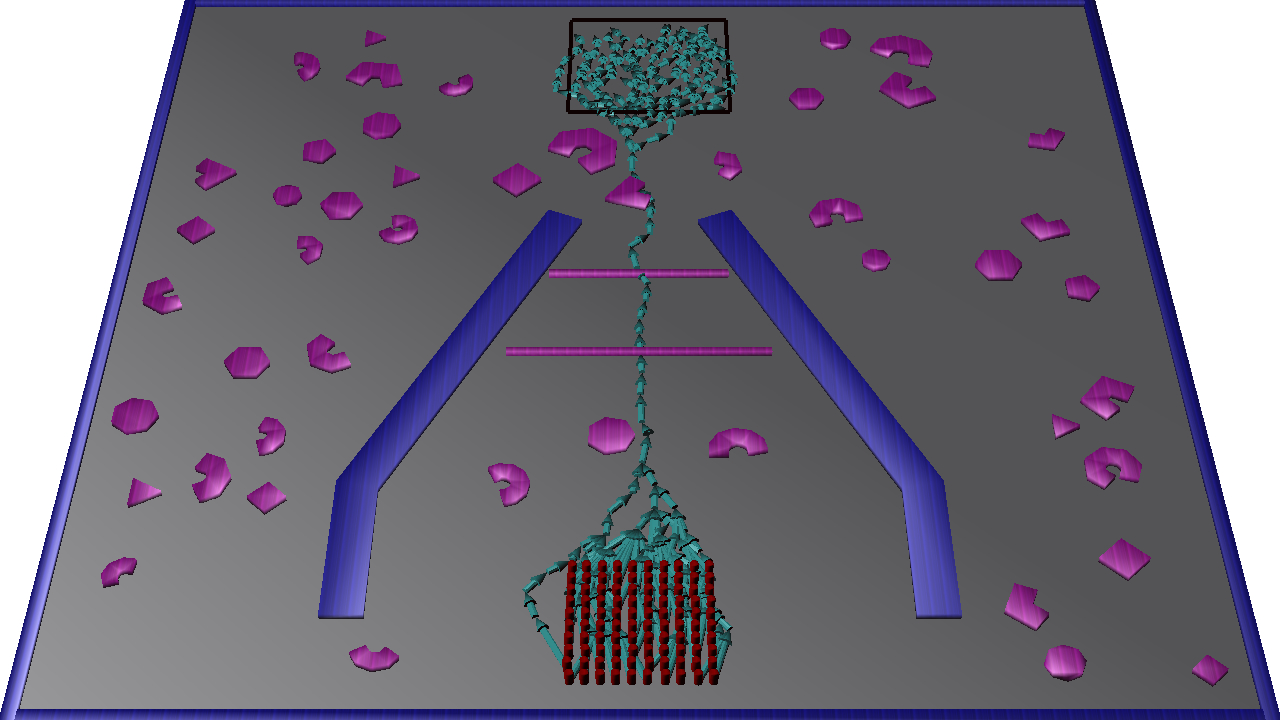
\includegraphics[width=0.32\linewidth]{figs/dcrops1}
    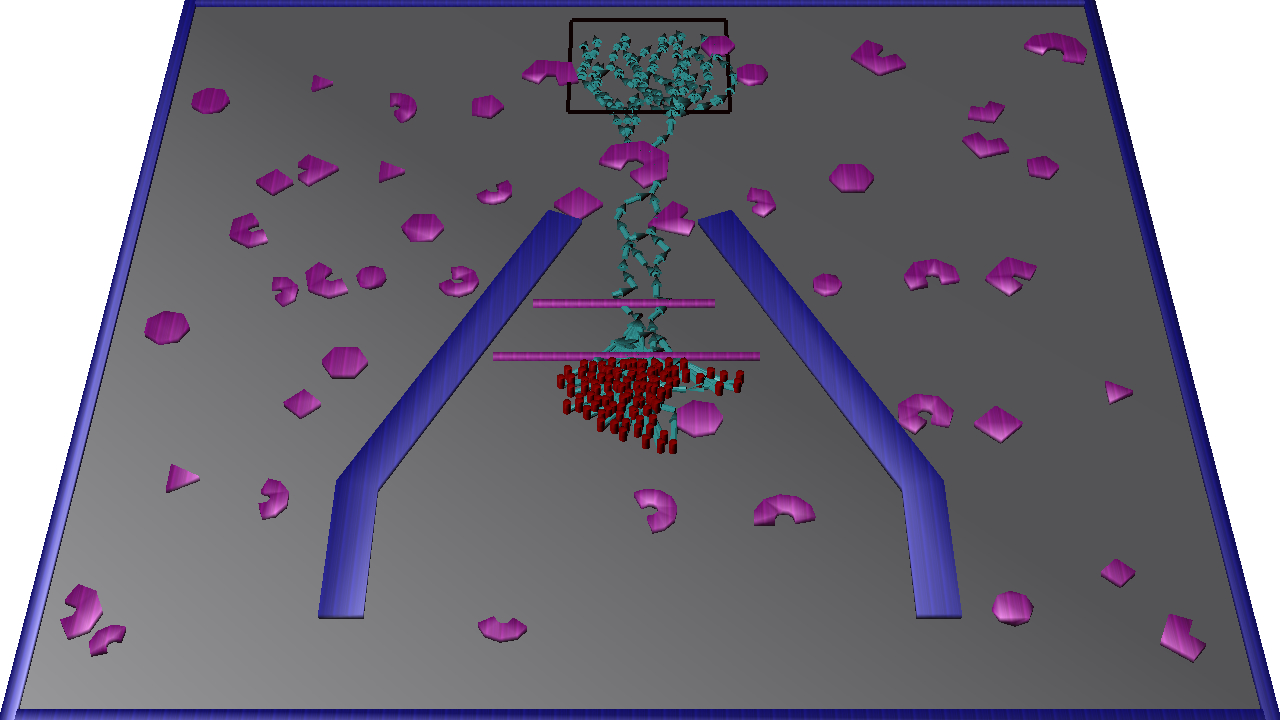
\includegraphics[width=0.32\linewidth]{figs/dcrops2}
    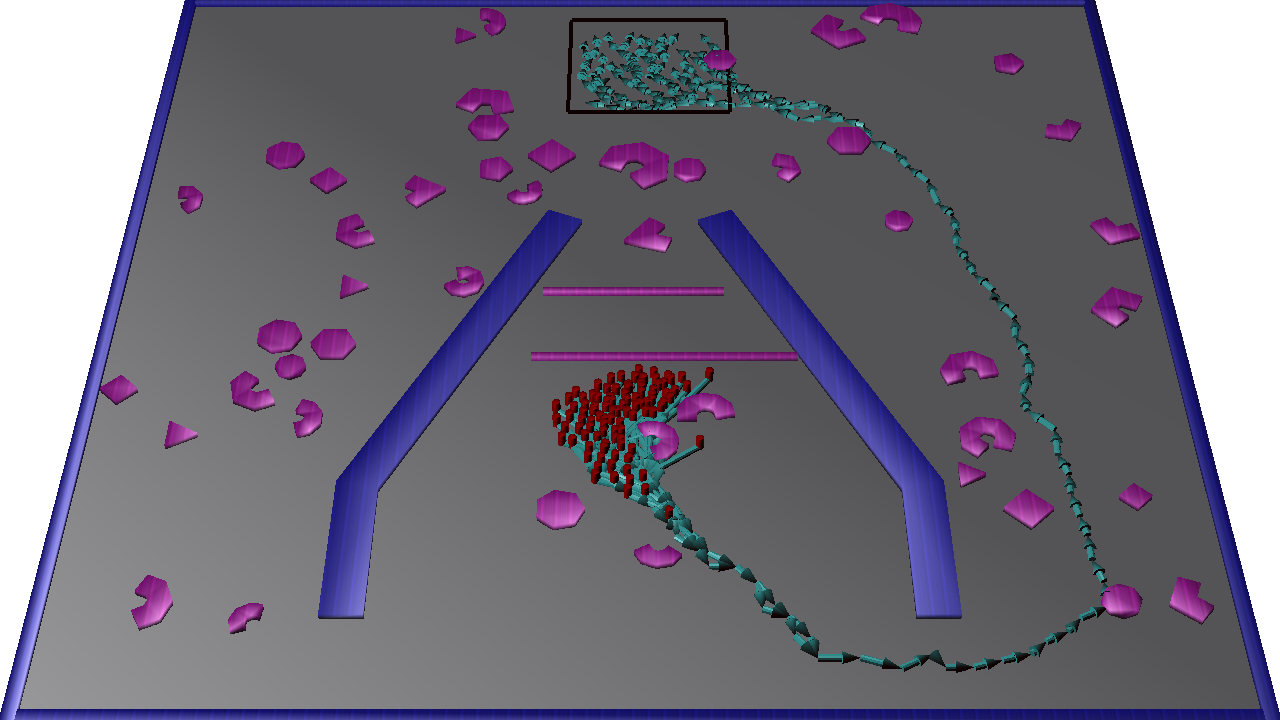
\includegraphics[width=0.32\linewidth]{figs/dcrops3} \\[2mm]
    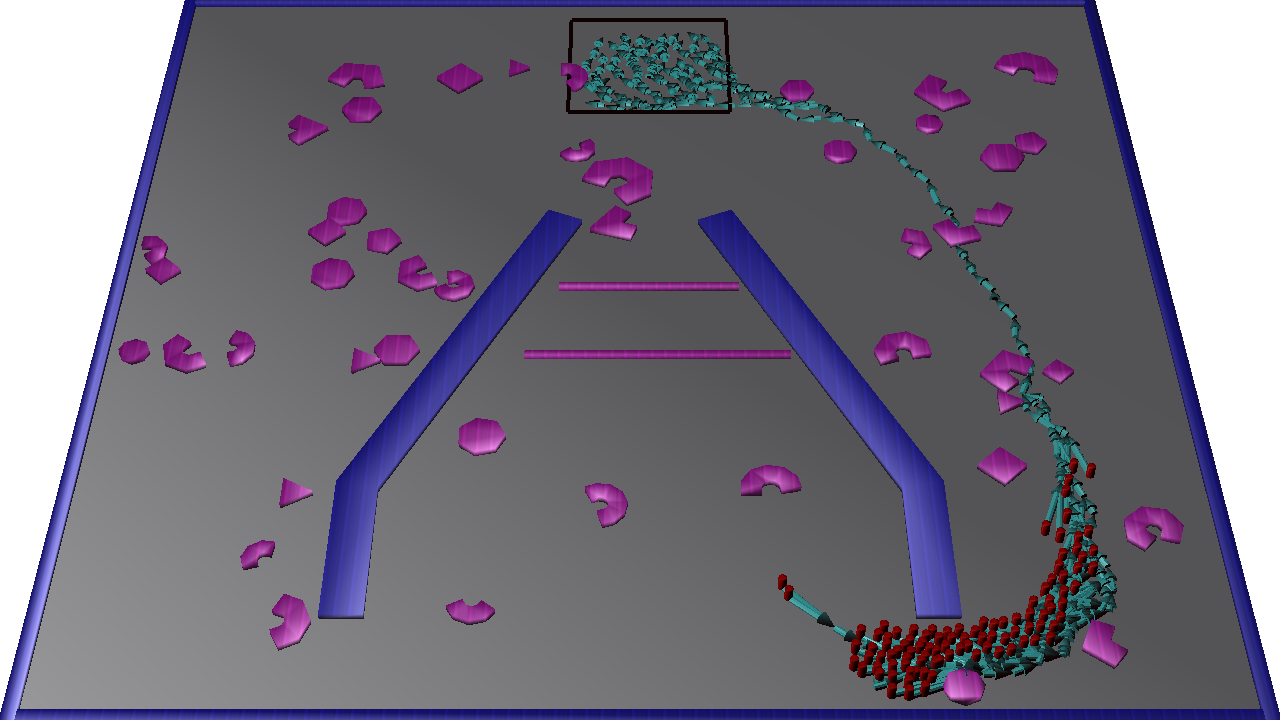
\includegraphics[width=0.32\linewidth]{figs/dcrops4}
    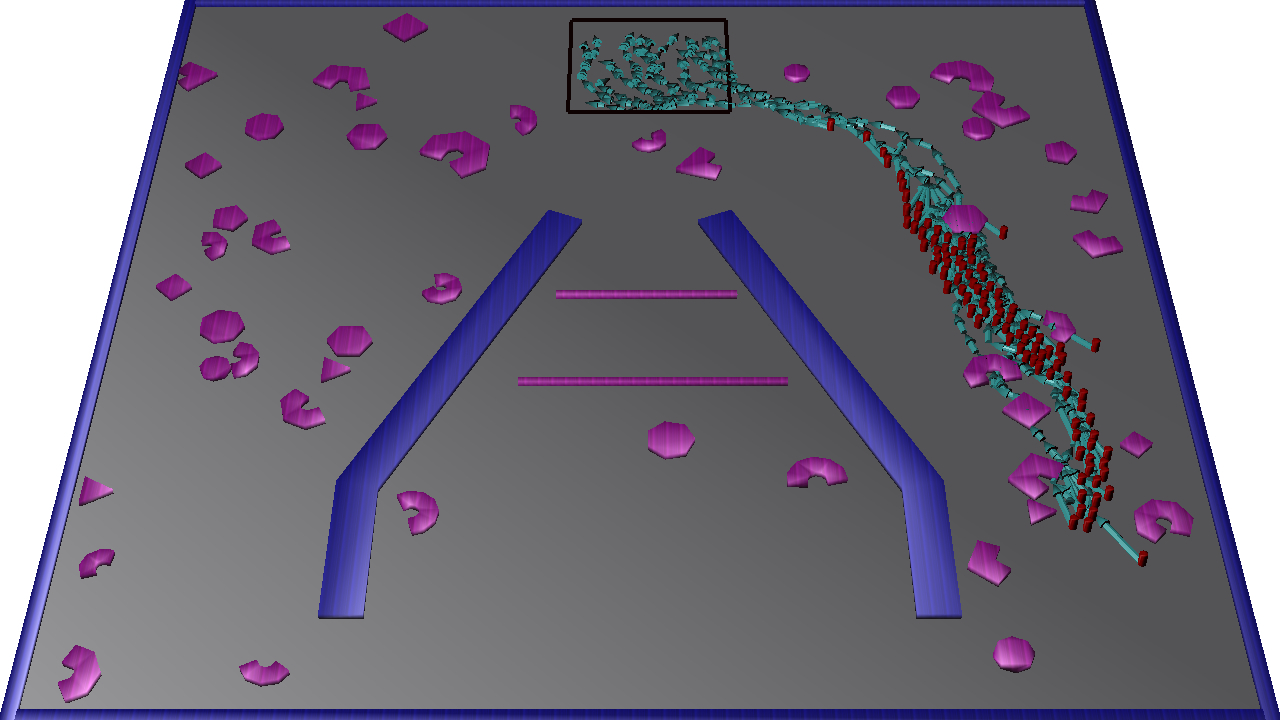
\includegraphics[width=0.32\linewidth]{figs/dcrops5}
    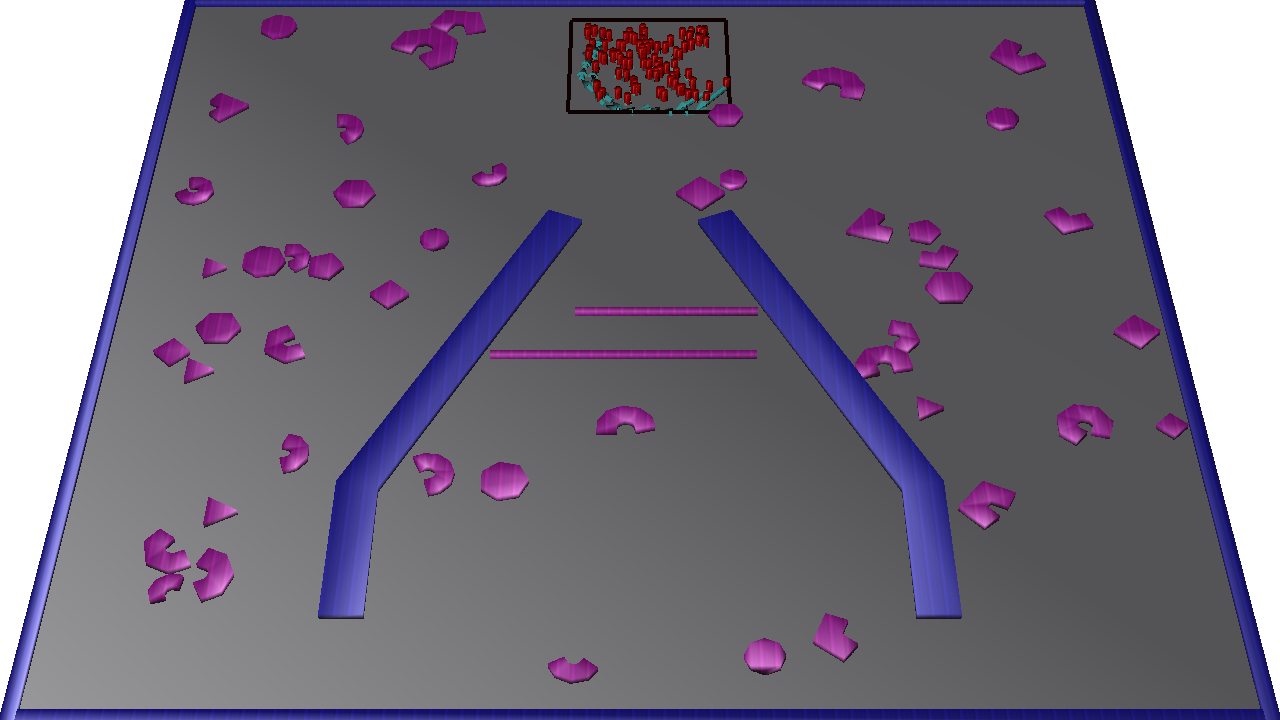
\includegraphics[width=0.32\linewidth]{figs/dcrops6}

    \caption{Planning the movements of a swarm by using a probabilistic roadmap
        as a global planner and potential fields as a local planner. Notice how
    the swarm is able to re-plan the global path when a blockage formed by
dynamic obstacles is present.}

    \label{fig:dcrops}

\end{figure}

\subsection{Multi-Agent Risk-Sensitive Aerial Surveillance~\cite{parcov, rover}}

Autonomous teams of unmanned aerial vehicles have been used by the military to
provide high quality, persistent surveillance of a given area. These robots
often are subject to external risk (i.e. detection by hostile agents, fire,
wind). Amidst this risk, these teams have to provide persistent high quality
sensory information of the area. The key motivation for my interest in
multi-agent surveillance is that multi-agent systems have fault tolerance built
into the architecture. A single robot or multiple robots may no longer be
functional, but the persistent coverage may still be possible. Having a swarm
of robots collaborating to provide surveillance speeds up the process, but
techniques have been designed that allow for agents to leave the swarm and
still allow the swarm to provide the necessary coverage. During my internship
in the summer of 2014 at the Naval Research Laboratory, I created an algorithm
that is based on simple local rules that is able to plan the motions of a swarm
to continuously provide this information whilst minimizing the potential risk
and maximizing the quality of the sensory information captured~\cite{parcov,
rover}. Planning the motions of the robots in three-dimensional space was
broken into two parts, planning in the $xy$ plane and planning for altitude.
Planning in the $xy$ plane was accomplished by giving the robots a simple rule,
move towards the area along the edge of the robot's sensor footprint that has
the best combination of the lowest risk and highest uncertainty. For
determining the altitude, the robot moves in the direction that would best
maximize the sensor quality whilst minimizing the risk. Tests have been run
using AscTec Pelican quadrotors that show the viability of the approach.

\begin{figure}[h!]

    \centering

    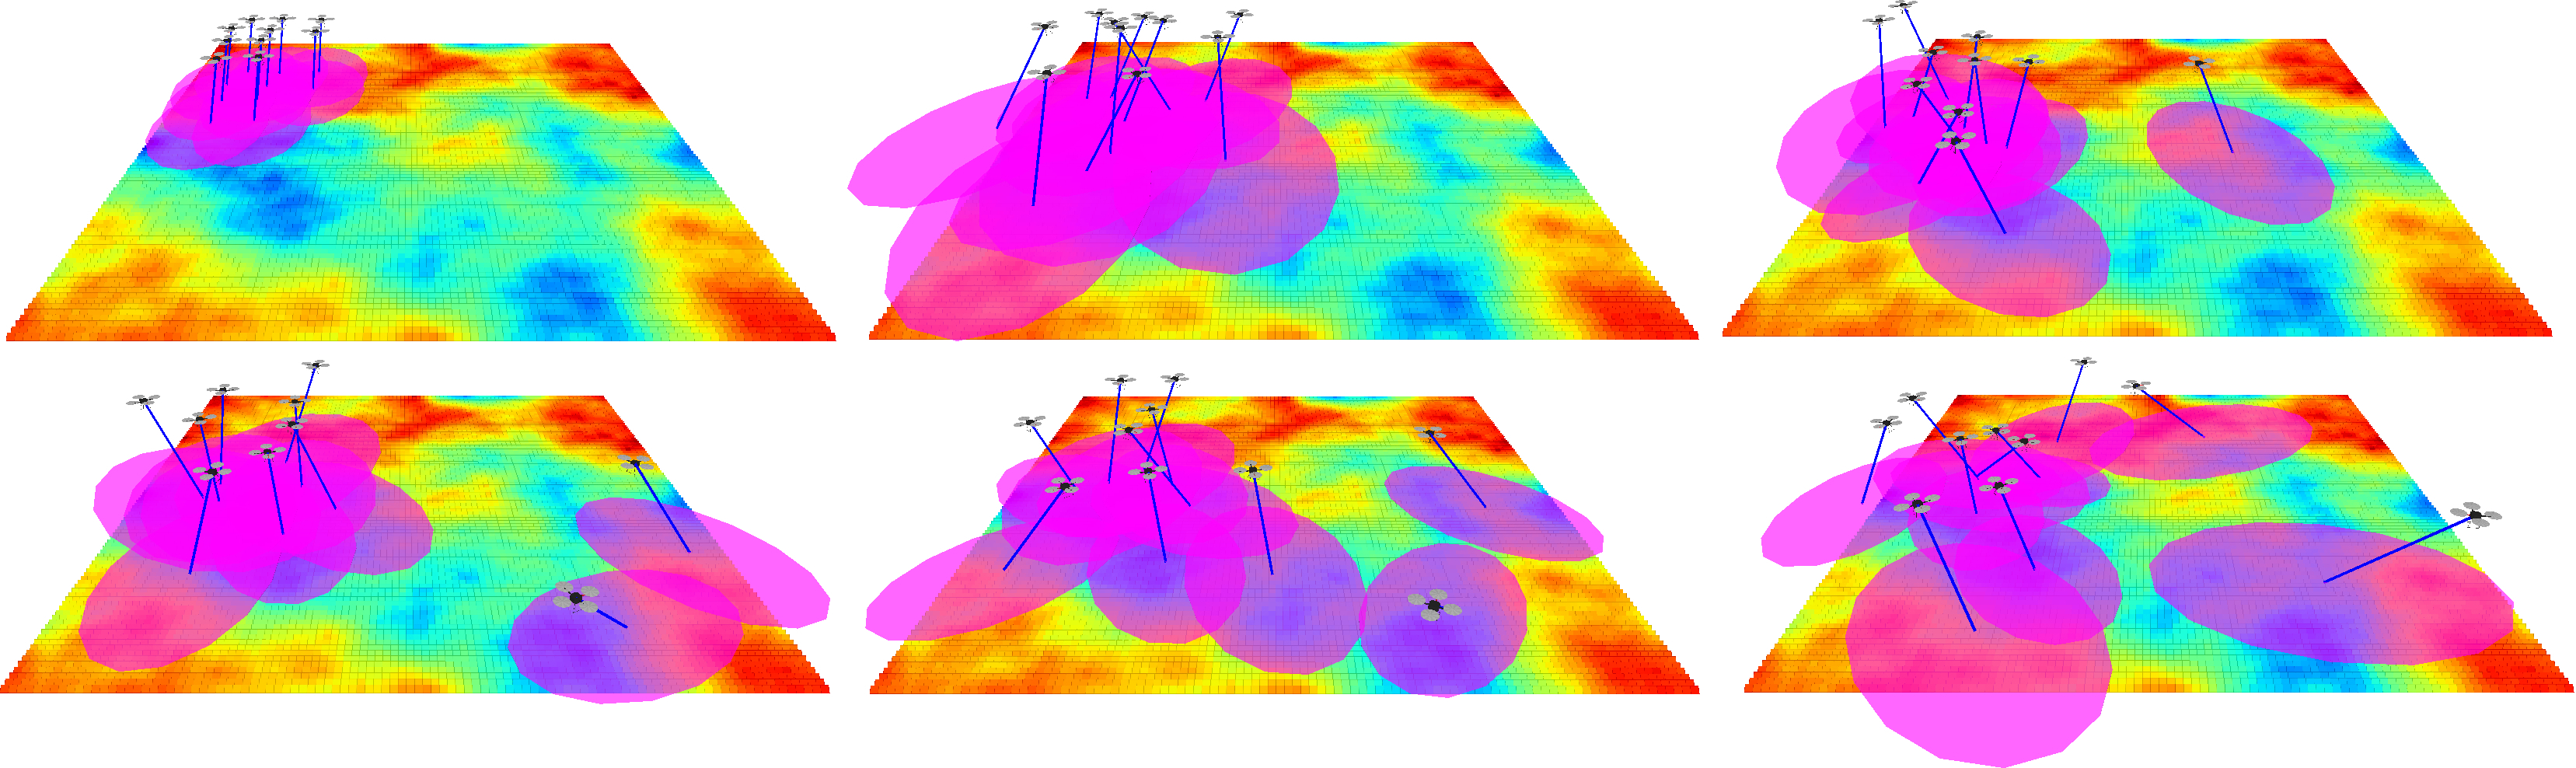
\includegraphics[width=\linewidth]{figs/rover}

    \caption{Using simple local rules to plan the trajectories of a swarm to
    provide persistent high quality sensory information of a given area whilst
minimizing the risk of gathering the information.}

    \label{fig:rover}

\end{figure}

\subsection{Multi-agent Source Localization~\cite{malt}}

There many occasions when localization of a particular stimulus source is not
possible with only one sensor node in the general case (i.e. heat, sound,
vibration, etc). Each of the sensor nodes receives non-directional information
about the intensity of the stimulus at their position. By combining the
knowledge from each of the nodes, we are able to determine the position of the
source. However, this case is only possible when there is no associated noise
with a given position in the search area. In real world scenarios there will be
noisy sensor readings and these could be caused either external or internal
perturbations. Averaging sensor intensities over time, removing outliers, can
account for noise caused by internal factors, but constant Gaussian noise based
on the location of the node must be accounted for by moving the node out of the
noisy area (i.e. for sound source localization, by moving out of locations with
high background noise). However in some cases it is not possible to determine
whether a node is in a noisy area (i.e. constant noise being applied to the
node) and therefore, consensus filtering is needed to determine how much noise
each node has and how to move the node out of the noisy area. As a
undergraduate research assistant at the Computational Robotics Group at the
Catholic University of America, I developed an algorithm that is able to
incrementally reduce the error in the location prediction for a source by a
group of mobile sensor nodes~\cite{malt}.  This is accomplished by moving the
sensor nodes at a speed inversely proportional to the amount they contributed
to the source localization during consensus filtering stage. The nodes move
towards the closest neighbour node that contributed the most to the
localization (i.e. the node that had the least agreed upon error during the
consensus filtering stage). This simple homogeneous rule for the swarm of
sensor nodes allows the global localization error to be reduced over time.

\begin{figure}[h!]

    \centering

    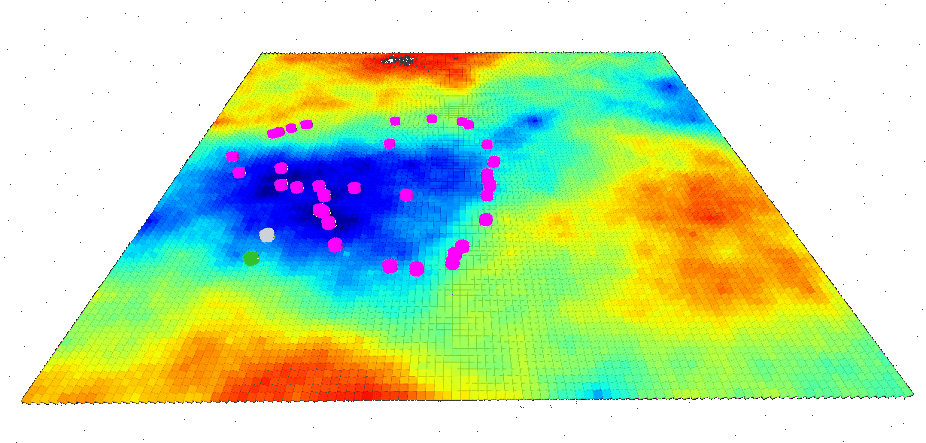
\includegraphics[width=\linewidth]{figs/malt}

    \caption{By moving nodes towards the neighbours with the smallest
    relative error, the predicted location of the source gets closer to the
location of the actual source. The red areas are areas of high noise whereas
blue areas have little noise.}

    \label{fig:malt}

\end{figure}

\section{Future Work}

Ultimately, my research aims to enable homogeneous or heterogeneous teams of
robots to accomplish high level objectives using very simple local rules. The
creation of simple rules for emergent behavior has the possibility of
addressing problems not only within my research domain, but also to further the
progress of amorphous computing and nanomedicine.

I plan to continue research in swarm robotics by developing algorithms using
simple local rules that create emergent behaviors that can complete several
higher level objectives such as search and rescue, autonomous surveillance, and
source localization. I would like to not only provide validation through
simulated environments, but to also test the developed algorithms on physical
robots in real-world situations. Furthermore, I would like to use tools such as
UPPAAL, SPIN, and PRISM to formally verify that the developed algorithms
function as expected.

For future research, I would like to extend the work I have done in multi-agent
autonomous surveillance to deal gracefully with heterogeneous teams of robots
capable of efficiently gathering different types of high quality sensory
information whilst minimizing risk (i.e. UAVs providing aerial imagery whilst
ground robots use this imagery to gather soil samples). I would also like to
create algorithms that optimize the number of robots needed in the field to
provide persistent coverage. For instance, a robot will eventually to to return
to a base station to recharge. At this time another robot can leave the base
station and take its place. Developing methods that determine the total number
of robots needed to survey an area 100\% of the time given the resources of a
base station (i.e.\ number of recharge stations) can lead to fully autonomous
persistent surveillance solutions that can be deployed with minimal oversight
in the field.

\begin{figure}[h!]

    \centering

    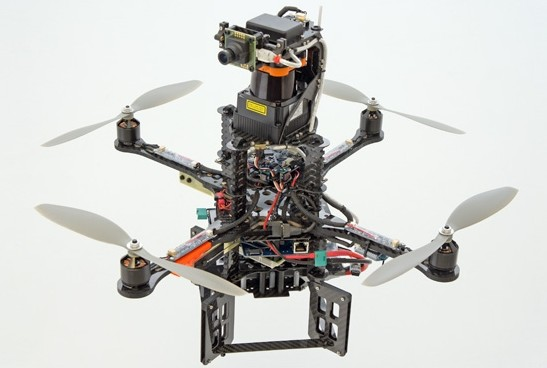
\includegraphics[width=0.6\linewidth]{figs/bird}

    \caption{An AscTec Pelican. The physical UAV that was used to test the
    risk-sensitive surveillance algorithms that were developed.}

\end{figure}

Furthermore, I am interested in expanding the multi-agent source localization
tool-kit I created to be more accurate by using genetic algorithms to
automatically generate neural controllers that are able to deal with the lack
of information provided by the system.

For my PhD, I would like to develop a set of algorithms that will allow a group
of robots to complete high level objectives with minimal human oversight or
intervention. These algorithms would allow the robots to return to base
stations to automatically recharge and dump gathered information and would
automatically optimize how many robots are in the field at any given time to
ensure persistent operation.

\bibliographystyle{ieeetr} \bibliography{proposal}

\end{document}
